% .:: Laden der LaTeX4EI Formelsammlungsvorlage
\documentclass[fs]{latex4ei}

% .:: Kopf- und Fußzeile
% ======================================================================
\usepackage{fancyhdr}
\pagestyle{fancy}
\fancyhf{}

   \fancyfoot[C]{von Emanuel Regnath}
   \renewcommand{\headrulewidth}{0.0pt} %obere Linie ausblenden
   \renewcommand{\footrulewidth}{0.1pt} %obere Linie ausblenden

   %\fancyfoot[R]{Stand: \todayV \ um \thistime \ Uhr \qquad \thepage}
   \fancyfoot[L]{Homepage: emareg.de - Fehler bitte sofort melden.}
	

% Dokumentbeginn
% ======================================================================
\begin{document}


% Aufteilung in Spalten
\begin{multicols}{4}

\fstitle{Computersysteme 1}

% ---------------------------------------
% | 		Computersysteme 			|
% ~~~~~~~~~~~~~~~~~~~~~~~~~~~~~~~~~~~~~~~
%=======================================================================

	\section{Hardware}
	BIOS = Basic Input Output System: Hardwarecheck, Simple Displayansteuerung\\
	ALU = Arithmetic Logical Unit
	CPU = Central Processing Unit
	GPU = Graphical Processing Unit
	RAM = Random Access Memory
	GPR = General Purpose Register
	SPR = Special Purpose Register
	
	
	\subsection{Grafikkarte}
	Bestnandteile: Speicher, GPU, BIOS, Shnittstellen\\
	VGA: R, G, B, Hsync, Vsync\\
	Antialiasing: Berechnung der prozentualen Farbintensitäten bei Farbüberdeckung.\\
	Front- und Backbuffer für Flickerfreie Darstellung.\\
	Aufgabe: Viele elementare Operationen parallel möglich. 

	\subsection{Optisches Laufwerk}
	Land: Oberfläche, Pits: Vertiefungen.\\
	Konstruktive bzw. Destruktive Interferrennz an den Vertiefungskanten.\\
	EFM = Eight-to-Fourteen-Modulation. 14Bit statt 8Bit pro Byte nötig.\\
	Multilayer: Halbtransparente und reflektierende Datenschicht.\\
	Brenner: Nichtrefkletierende Schicht und unterschiedliche Intensitäten.
	
	\subsection{Festplatte}
	Permanent- und Elektromagnet für Schwenkarm.\\
	Lesekopf Elektromagnet mit Ferritkern.\\
	Informationsspeicherung durch Länge der Magnetfeldlinien.\\
	Übereinanderliegende Spuren bilden einen Zylinder (parallele Schreib- und Lesevorgänge)\\
	
	\subsubsection{Ein Sektor 512 Byte Nutzdaten}
	60Byte Verwaltung: Sync des Taktes, Prüfsummen (CRC)\\
	Nummer des aktuellen Zylinders/Sektors/Lesekopf.\\
	Start und Endmarken für Datenbereich
	"Leer-Byte" als Tolranzzone



	\subsection{Assemblerebene}
	Register: schneller Datenspeicher, welcher genau ein Wort abspeichern kann.\\
	Es gibt allgemeine und spezielle Controll-Register \texttt{CR0, CR1, ...}
	Wort: Datenbreite die ein Prozessor auf einmal bearbeiten kann.\\
	RAM: Speichert einzelne Bytes.
	Adressierung: Big Endian: speichert MSB, Little Endian: speichert LSB (Intel)


	Anzahl der Operanden:\\
	Dreiadressmaschine:  \$1 $\leftarrow$ \$2 + \$3\\
	Zweiadressmascine: \$1 $\leftarrow$ \$1 + \$2\\
	Einadressmaschine: A $\leftarrow$ \$1 + A\\
	Nulladressmascine: Stack-Maschine\\

	Architekturen:\\
	CISC: Complex Instruction Set Computer (veraltet)\\
		kurze ,einfache Programme | lange Taktzyklen, kein Piplining.\\
	RISC: Reduced Instruction Set Computer (vorherrschend)\\
		einfache, gleich lange Befehle | mehr Speicher
	

	\section{Rechneraufbau}
	Peripherie -- EAP -- BUS -- CPU -- BUS -- Speicher\\
	\\
	Programmieren: Hochsprache(C++) $\ra$ Assemblercode(ASM) $\ra$ Maschinencode\\
	Gesetz von Amdahl: Optimierung wirkt sich nur im Verhältnis der Häufigkeit eines Programmteils auf die Gesamtlaufzeit aus.\\
	$\Ra$ Optimiere die am häufigsten vorkommenden Programmteile.
	



\section{MMIX Architektur}
Hypothetischer $\mu$C von Donald Knuth für Lehrzwecke\\
Load-Store Architektur: Nur GPR mit ALU verbunden.\\
256 Register(32 SPR), 64Bit Wortbreite, 256 Befehle (1 Takt)\\
Big-Endian Adressierung\\	
	
	\subsection{Register}
	\texttt{\$0 $-$ rL-1}: lokale Register,\\
	\texttt{rL $-$ rG-1}: marginale Register(unentschieden)\\
	\texttt{\$255 $-$ rG}: globale Register\\
		
	\subsection{Hauptspeicher (RAM)}
	Text\_Segment: 256Byte Interruptvektoren, Programmcode\\
	Data\_Segment: Für Daten(unten) und Stack(oben)\\
	Pool\_Segment, Stack\_Segment, Betriebsystembereich\\
	\\
	Speicherzugriffe: Byte(1), Wyde(2), Tetra(4), Octa(8)\\
	Big-Endian: Adressen zeigen auf MSB (MMIX)\\
	Little-Endian: Adressen zeigen auf LSB\\	

	\subsection{Programmloader}
	Der Programmloader läd das Programm (führt den Befehl LOC aus)
	und such nach der \texttt{Main}-Marke bei der das Programm startet.

	
	\subsection{Befehle}
	Format: \texttt{Marke BEFEHL \$1,\$2,\$3 Kommentar}\\
	$\Ra$ Max. 3 Leerzeichen pro Zeile, Operanden nur durch Komma getrennt.
		
		\subsubsection{Wichtige Befehle}
		\begin{tabular}{ll}
			\texttt{LOC Adresse} & Nachfolgende Befehle ab \texttt{Adresse} ausführen\\
			\texttt{GREG Adresse} & Schreibt \texttt{Adresse} in Globales Register\\
			\texttt{BYTE Wert} & Reserviert 1 Byte, initialisiert mit Wert\\
			\texttt{SETL \$X,YZ} & Setzt Bits 0--15 von \texttt{\$X} auf \texttt{YZ}\\
			\texttt{LD$\square$ \$X,\$Y,(\$)Z} & Lade $\square$ von Adr. \texttt{\$Y+(\$)Z} in Reg. \texttt{\$X} \\
			\texttt{LDA \$X,Label} & Lade Adr. von \texttt{Lable} in Reg. \texttt{\$X}\\
			\texttt{ST$\square$ \$X,\$Y,(\$)Z} & Speichert Reg. \texttt{\$X} in Adr. \texttt{\$Y+(\$)Z}\\ 
			\texttt{JMP Label} & Springt zu \texttt{Label}\\
			\texttt{GO \$0,Label} & Springt zu \texttt{Label} und speichert Folgeadr. in \texttt{\$0}\\
			\texttt{CMP \$X,\$Y,(\$)Z} & Vergleich; \texttt{\$X = sgn(\$Y - (\$)Z)}\\
			\texttt{TRAP 0,Halt,0} & Beendet das Programm\\
		\end{tabular}
	LD$\square$U: vorderen Bits werden mit Nullen gefüllt\\
	LD$\square$: vordere Bits werden mit Vorzeichen gefüllt\\
	$\square$=B(Byte/8b), W(Wyde/16b), T(Tetra/32b), O(Octa/64b)\\

		
		\subsubsection{Arithmetik}
		\begin{tabular}{ll}
			\texttt{ADD \$X,\$Y,(\$)Z} & \texttt{\$X = \$Y / \$Z}\\
			\texttt{SUB \$X,\$Y,(\$)Z} & \texttt{\$X = \$Y - \$Z}\\
			\texttt{MUL \$X,\$Y,(\$)Z} & \texttt{\$X = \$Y * \$Z}\\
			\texttt{DIV \$X,\$Y,(\$)Z} & \texttt{\$X = \$Y / \$Z}\\
		\end{tabular}	
		
		\subsubsection{Verzweigung und Bedingungen}
		\begin{tabular}{ll|l}
		Branch & \texttt{B- \$X,Label} & Springt zu \texttt{Label} if \texttt{\$X} \\
		Conditional Set & \texttt{CS- \$X,\$Y,(\$)Z} & \texttt{\$X = \$Z} if \texttt{\$Y} \\
		Zero or Set & \texttt{ZS- \$X,\$Y,(\$)Z} & \texttt{\$X = \$Z} if \texttt{\$Y} else \texttt{\$X = 0}\\ 
		\end{tabular}\\
		\begin{tabular}{ll|ll}
			\texttt{-Z} & if Zero & \texttt{-NZ} & not zero\\
			\texttt{-P} & if positive & \texttt{-NP} & not positiv\\
			\texttt{-N} & if negative & \texttt{-NN} & not negative \\
		\end{tabular}	
		
		
		
	

	Jeder Befehl hat 32 Bit:\\
	\framebox[1.0cm]{OPC}\framebox[1.0cm]{\#\$1}\framebox[1.0cm]{\#\$2}\framebox[1.0cm]{Offset}\\
	\\
	Laden: RAM $\ra$ Register, Speichern: Register $\ra$ RAM\\ 
	\\
	Namensraum: \texttt{PREFIX Prefix:} Vor alle Labels wird \texttt{Prefix:} geschrieben\\
	Globale Labels mit : davor: \texttt{:Main}\\
	Namensraum beenden: \texttt{PREFIX :}\\



	\subsection{ALU – Arithmetic Logical Unit}
	
	
		\subsubsection{Schieber}
		Steuerung: 00,01,10,11 für SL,SLU,SR,SRU; \quad nur SL liefert Überlauf!\\
	
		\subsubsection{Division}
		$\underset{\text {Dividend}}{a_1 a_2 a_3 ...} / \underset{\text {Divisor}}{b_1 b_2 b_3 ...} = \underset{\text {Quotient}}{c_1 c_2 c_3 ...}$\\
		Wie bei Basis Zehn, nur dass Divisor maximal einmal abgezogen werden muss.
		Statt Divisor nach rechts schieben, Rest nach links schieben.\\

		Ablauf: 
		1. Dividend in Restregister ablegen\\
		2. Divisor in linker Hälfte des Divisorregisters ablegen.\\
		3. Divisor = Divisor $>>$ 1\\
		4. Quotient = $<<$ 1\\
		5. Rest = Rest $-$ Divisor\\
		
		6543/21
		\begin{tabular}{ll|l}
		Restregister: & 0000 & 6543\\
		Divisorregister: & 0021 & 0000\\
		\end{tabular}
		Restregister = Ergebnisregister (Rest links, Erg rechts)\\
		
		\$X$\mod n$: {\tt DIV \$X,\$X,n \qquad GET \$X,rR}\\
		\texttt{if \$Y $\circ$ \$Z: SUB buf,\$Y,\$Z \qquad B(N)P/N buf,Label}\\
		
		
		\subsection{Stack}
		Initialisieren des Stacks:\\
		\begin{tabular}{lll}
			\texttt{BOS} & \texttt{GREG Pool\_Segment} & Bottom-Of-Stack \\
			\texttt{SP} & \texttt{GREG Pool\_Segment} & Stackpointer \\
		\end{tabular}\\
		Bsp: Push und Pop von zwei Registern {\tt a} und {\tt b}:\\
		\begin{tabular}{l|l|l}
			& Push & Pop \\ \mrule
		1. 	& \texttt{SUB SP,SP,2*8} & \texttt{LDO b,SP,0}\\
		2.	& \texttt{STO b,SP,0*8} & \texttt{LDO a,SP,1*8}\\
		3.	& \texttt{STO a,SP,1*8} & \texttt{ADD SP,SP,2*8}\\
		\end{tabular}\\
		\\
		Funktionsaufruf der Funktion \texttt{Fkt}: 
		\begin{enumerate}\itemsep0pt
			\item Variablen zur Übergabe auf den Stack speichern (Push)
			\item Sprung zum Funktionscode: \texttt{GO \$0,Fkt}
			\item Von \texttt{Fkt} benötigte Register auf dem Stack sichern (Push)
			\item Übergebene Variablen vom Stack in die Register laden (Pop)
			\item Berechnungen in den gesicherten Registern durchführen
			\item Übergabewert auf dem Stack mit Rückgabewert überschreiben (Push)
			\item Alte Registerinhalte wiederherstellen (Pop)
			\item Stackpointer auf die Adresse des Rückgabewerts setzen 
			\item Rücksprung \texttt{GO \$0,\$0,0}
		\end{enumerate}

\section{Zustandsautomaten}
Register: Haben immer aktuellen Wert am Ausgang, Änderung nur bei \texttt{clk}\\
\texttt{clk} Variablen mit steigender Taktflanke, müssen im vorherigen Zustand auf 0 gesetzt sein.\\
\texttt{Reset} Veriablen müssen meistens auf 0 gehalten werden.\\
 
		
		
\subsection{Programmierbare logische Anordnung PLA}
Eingänge $\ra$ Zustände (AND) $\ra$ Ausgänge (OR)\\



\section{Datenpfade}
Die 5 Phasen der Befehlsausführung:\\
\begin{enumerate}\itemsep0pt
	\item BH: Befehl holen (IF = Instruction Fetch)
	\item BD: Befehl dekodieren (ID = Instruction Decode)
	\item AF: Befehl ausführen (EX = Execute)
	\item SP: Speicherzugriff (MEM = Memory Access)
	\item ES: Ergebnis schreiben (WB = Write Back)
\end{enumerate}


\subsection{Piplining}
Trennung von sequentiellen Elementen durch Register. $\Ra$ Einzelelemente Parallelisierbar.\\
Datendurchsatz steigert sich max. um Faktor $S$: $D' = S \cdot D$\\
Max. Taktrate entspricht dem Kehrwert der Ausführungszeit der langsamsten Stufe: $f_{max} = \frac{1}{t_{max}}$\\

	\subsubsection{Datenkonflikte}
	Generell keine Konflikte falls $\ge$ 3 Befehle dazwischen!\\
	Zwischen ES und BD: beim schreiben/lesen von \$$X$\\
	Zwischen ES und AF: beim rechnen mit nicht gespeicherten Werten (kann durch Stall gelöst werden)
	
	Zwischen \texttt{LD$\square$ \$X,*,*} und \texttt{ST$\square$ \$X,\$Y,\$Z}\\
	Nicht zwischen \texttt{ST$\square$ *,\$Y,\$Z} und \texttt{LD$\square$ *,\$Y,\$Z}
	
	
	Stalls nötig falls direkt nach einem \texttt{LD$\square$}-Befehl das Zielregister \texttt{\$X} für Berechnungen in der AF Phase benötigt wird.\\
	Sonst kann der Konflikt durch einen Forward-Pfad gelöst werden.\\


	\subsubsection{Strukturkonflikt}
	Gleichzeitiges Lesen und Schreiben im Registerblock.\\
	Tritt auf, falls 3 Befehle vor \texttt{ST$\square$} das Register \texttt{\$ X} gelesen wird.\\
	
	
	\subsubsection{Steuerungskonflikt}
	Direkt nach einer Registerneuzuweisung(\texttt{ADD \$X,\$Y,\$Z}) wird ein durch dieses Register bedingte Operation ausgeführt(\texttt{BNZ \$X,Label}). 
	Dadurch ist nicht definiert welcher Befehl als nächstes kommt. Lösung: Befehlsumstellung,Stalls\\
	 

\section{Speicher}
Register -- Cache -- Hauptspeicher -- Festplatte\\


\subsection{Cache}
 \boxed{ \text{4MB:} 2^{22} \text{bit} }\\
besteht aus $s$ Sets mit jeweils $r$ Rahmen mit jeweils $B$ einzelnen Bytes.\\
Tag = Adresse der Daten im Speicher\\
Valid-Bit: Daten im Cache sind gültig


\boxed{\text{\#Schlüsselbits} = \text{Bandbreite} - \text{\#Setbits} - \text{\#Bytebits}}


Direct Mapped Cache:\\


Fully-Associative-Cache:\\



Set-Associative-Cache:\\
$\text{\#Speicherbits} = \text{\#BAbits} + \frac{\text{\#Rahmenbits}}{\text{Set}} + \text{\#Setbits}$ \\
Rahmengröße = $2^BA$\\
Ein Rahmen pro Set\\


$\frac{\text{\#Zugriffe}}{\text{Zeit}} = \text{Hit-Rate} \cdot \text{Hit-Time} + \text{Miss-Rate} \cdot \text{Miss-Time}$ \\













% -------------------------------------------
% | 		Computersysteme 2				|
% ~~~~~~~~~~~~~~~~~~~~~~~~~~~~~~~~~~~~~~~~~~~
%=======================================================================
	\newpage
	\parbox{4cm}{
		\emph{\Large{Computersysteme 2}}
	}

Apps -- OS -- Hardware\\
Betriebsystem: Grundsoftware zum ausführen, steuern und überwachen von Programmen.\\
System: Von der Umwelt mit Schnittstelle getrennte Menge an verknüpften Komponenten.\\

Begriffe:\\
\begin{tabular}{lp{4.5cm}}
	busy waiting & Warten auf Ereignis mit ständiger Nachfrage\\
	Mutal exclusion & Zugriffe auf gemeinsame Variable hintereinander\\
	Race-Condition & Parallele Prozesse lesen und schreiben in gemeinsamer Variable.\\
	SRPT & Shortest-Remaining-Process-Time (PV Strategie)\\
	LCFS & Last Come First Served (PV Strategie: )\\
	ELF & Executable and Linking Format (Ausführbare Dateiformat)\\
	MMU & Memory Management Unit\\

\end{tabular}

\section{Betriebsmittel BM}
Klassifizierung: \\
Entziehbarkeit: unterbrechbar(UBM)/ununterbrechbar(DBM)\\
Wiederverwendbarkeit: einmalig(EBM)/wiederholbar(WBM)\\
Exklusivität: parallel benutzbar(PBM)/exklusiv(XBM)/teils(BBM)\\



Virtueller Speicher(4GB bei 32Bit): ca. 1GB für BS; 3GB für Code, Stack, Heap...\\ 

\section{Prozesse}
$\approx 100$ Prozesse aus $\approx 1000$ Threads laufen im Hintergrund von Windows/Linux.\\
User- und Systemmodus (mit previligierten Befehlen)\\
Zustände: running und ready\\
Verteilung der Rechenzeit an die Prozesse:\\
Scheduler: Verwaltet die Priorität von Prozessen. (Akt. neuen P)\\
Dispatcher: Schaltet Prozesse um. (Akt. Interrupts)\\
\\
{
\framebox{\parbox{6.0cm}{
\begin{tabular}{lr}
	POSIX & API\\
\end{tabular} }}\\	
\framebox{\parbox{6.0cm}{
\begin{tabular}{c|c|c}
Pförtner & Shell & \\ \mrule
EA & Dateisystem & Prozessverwaltung \\ \mrule
Unterbrechungen & Prozessschedule & \\
\end{tabular}}}
\framebox{\parbox{6.0cm}{
	Hardware }}
}

\begin{tabular}{llll}
	Jahr & Technologie & BS & Sonst\\
	1945 & Röhren & -- & Ein Benutzer\\
	1955 & Transistoren & IBM & Lochkarten\\
	1965 & ICs	& OS 360 & Multitasking\\
	1970 & LSI & Unix & Dateisystem\\
	1980 & $\mu$C & Mirosoft & PC\\
\end{tabular}



UNIX-Scheduler: Round-Robin Zeitscheibenstrategie mit 100ms
Quellcode $\xrightarrow{\text{Compiler}}$ Binäre Objektdatei.o (Code + Daten)\\
Objektdatei\emph{en} + Bibliothek\emph{en} $\xrightarrow{\text{Linker}}$ Eine Executable\\
Executable $\xrightarrow{\text{Loader}}$ Prozess im RAM\\
ELF: Relocateable Files.o, Executable Files, Shared Object Files.so\\




\subsection{Semaphore (Koordinationsvariable) $m$}
Leser-Schreiber Problem:
Es dürfen beliebig viele Leser auf eine Datei zugreifen solange niemand schreiben will.\\
Sobald ein Prozess in die Datei schreibt, werden neue Leser in die Warteschlagen gesetzt.
Attribut, dass für beschränkte Ressourcen zur Zugriffskontrolle verwendet wird.
Zunächst gilt $m = 1$, will jemand Datei beschreiben $m = m-1$\\
falls $m = 0 \Ra$ Zugriff, falls $m < 0 \Ra$ warten\\
wenn Schreibvorgang fertig, dann $m = m +1$\\


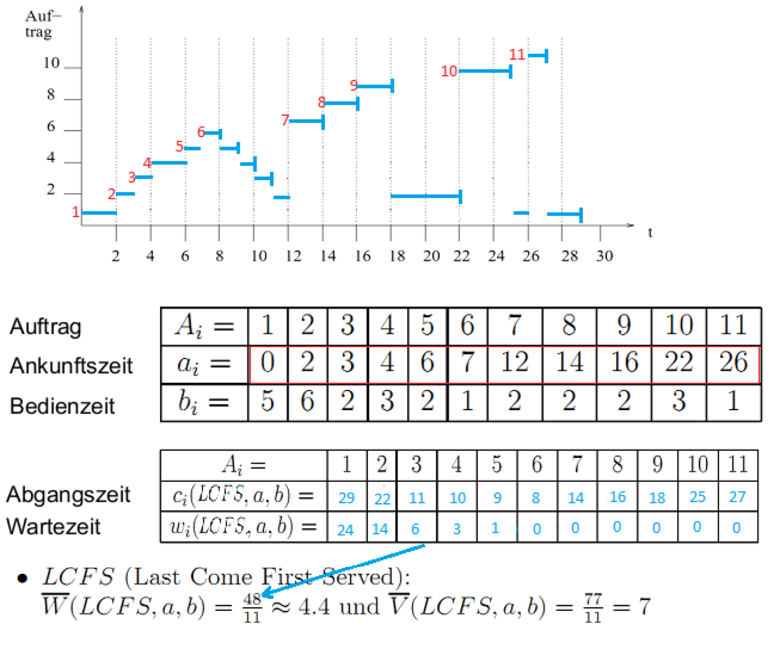
\includegraphics[scale = 0.5]{./img/Prozessorverwaltung.pdf}


\subsection{Deadlocks (Verklemmung)}
Def: Es gibt keinen Ablauf, so dass alle Forderungen nach Ressourcen erfüllt werden können.\\
Mind. zwei Prozesse warten gegenseitig auf die Freigabe der jeweils anderen Ressource.\\
Notwendige Bedingungen:
BM ist exlusiv, BM is nicht entziehbar, Belegen und Anfordern, Zyklisches Warten\\ 
Lösungen: Ignore, Discover/Recovery, Avoidance (Verhinderung: Sorgfältige Zuweisung), Prevention (Vermeidung einer Bedingung)\\

Beispiel: Zwei Leute wollen etwas schreiben, der eine hat den Stift, der andere das Papier.\\
Wechselseitiger Ausschluss mit aktiven Warten kann zu Deadlocks führen, wenn der Prozess nicht unterbrochen werden kann.\\
Lösung: Passives Warten: Prozess wird vom Besetzer einer Ressource aktiviert wenn dieser sie nicht mehr benötigt.\\


\subsection{Linux}
Prozesse haben unterschiedliche Berechtigungen.\\
Priviligierte Aufrufe im Nicht-priviligierten Modus: systemcalls\\
Schutzkern: Fälschungssichere Objekt-IDs, Rechteverwaltung\\
Rechte: read (r, 4), write (w, 2) und execute (x, 1)\\
Für Besitzer, Gruppe und Andere (chmod 764, chown ...)\\
Datei: Folge von Bytes(regular, directories, devices(/dev)\\
Pipe: FIFO Komunikationspfad zwischen Programmen.\\
Links: Softlink(Symbol zB Pfadangabe) Hardlink(Zweiter INode)\\
Platte: SWAP $|$ Inodes -- Datenblöcke(cluster) -- Reserveblöcke\\
Dateiverwaltung über INodes: ID, Typ, Rechte, Besitzer, Größe, Blöcke\\
Aufgabe Ausführung und Datenteile im Quellcode: Datenteile nur bei int,const, etc Befehlen!

Prozessstart:
\begin{enumerate}
	\item Header Infos auf der ersten Seite lesen
	\item Speicher allokieren
	\item Blende Sectionen in Adressraum ein
	\item Fehlende Biblitheken laden
	\item Initialisiere Stack und Heap
	\item Code ausführen
\end{enumerate}

Verwaltungsstrategien LRPT/SRPT \quad LPT/SPT \quad LCFS/FCFS\\
Permutationsverfahren und zwei Zeitscheibenverfahren\\
Auftrag $A_i$, Ankunftszeitzeit $a_i$, Bedienzeit $b_i$, Abgangszeit $c_i$, Wartezeit $w_i$\\
\boxed{ c_i - b_i = w_i + a_i }\\
$\overline W = \frac{1}{n} \sum w_i$ \quad $\overline V = \frac{1}{n} \sum w_i + b_i$\\


\section{Speicher}
Häufigkeit der Nutzung: MFU, LFU\\
Zeitpunkte der Einlagerung: FIFO, LIFO\\
Zeitpunkt der letzten Nutzung: LRU, MRU\\

\subsection{Virtueller Speicher VS}
Gliederung: Segmente $>$ Seiten $>$ Zellen\\
Stretegie: First Fit, Rotating First Fit, Best Fit und Worst Fit\\
page fault (Seitenfehler): Seite nicht mehr im phys. RAM\\
VS: Bessere Nutzung kann real auch auf HDD liegen. MMU notwendig.\\
Jede Anwendung erhält virtuellen, linearen Speicherbereich\\
Seitenersetzung: FIFO, LIFO, LRU, LFU\\
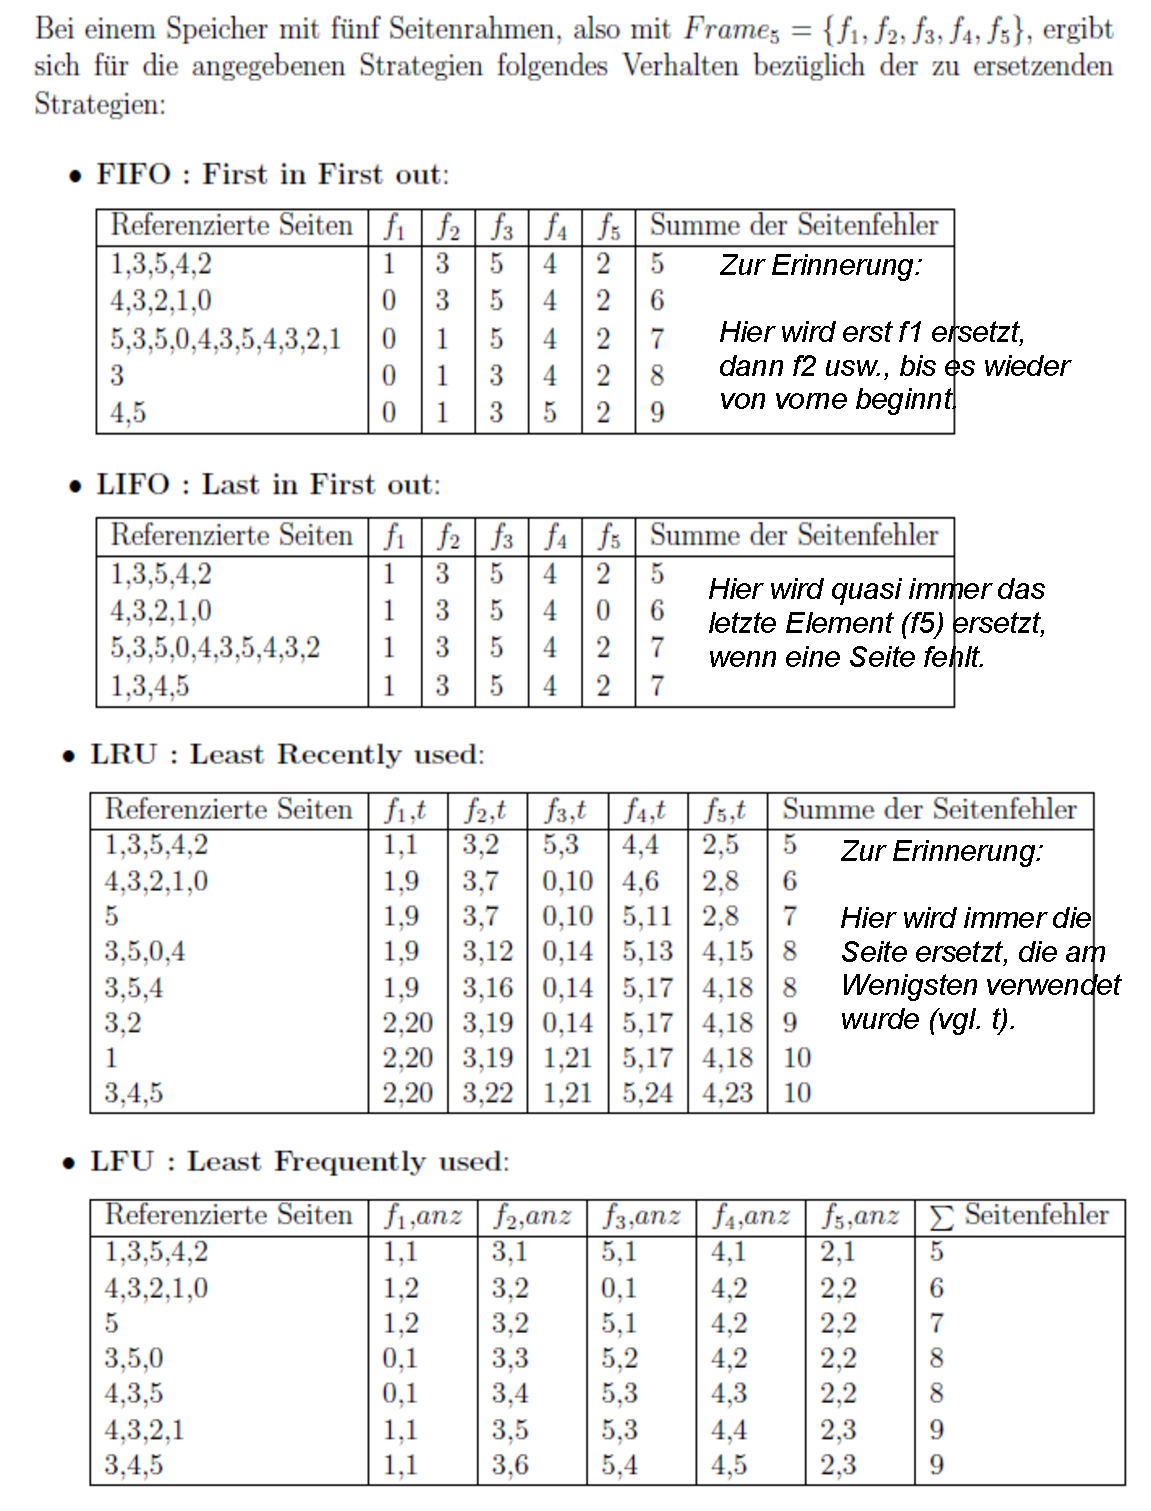
\includegraphics[scale = 0.35]{./img/VSLIFO.pdf}


\subsection{Datenbanken Systeme (DBS)}
Entity Relationship Modell (ER-M):\\
Rechteck: Objekte, Ellipse: Attribute, Raute: Methoden, Beziehungen\\
Schlüssel: Minimale Menge von Attributen, die ein Entity(Objekt) eindeutig in der Menge seiner Entities identifiziert (z.B. MatNR)\\

Datenbankentwurf:\\
\begin{itemize}
	\item Existenzabhängigkeit von Entities (schwache und starke Entities)
	\item Generalisierung und Spezialisierung
	\item $is-a$ und $part-of$ Beziehungen
	\item Verschiedene Sichten (Rechte, Zugriffe)
\end{itemize}

Das relationale Modell
Mengenorientierte Verarbeitung


\subsection{SQL Befehle}
\texttt{SELECT} * bzw. Attribut1, Attribut2,... (werden ausgegeben)\\
\texttt{FROM} Objekt1, Objekt2, ... (alle Benötigten Quellen auch von WHERE)\\
\texttt{WHERE} Bedingung1 \texttt{AND/OR} Bedingung2\\
\texttt{ORDER BY} Attribut1 (\texttt{DESC}), Atrribut2 \textbf{\large ;}\\
\\
Bedingung: (\texttt{NOT}) Attribut $=,<,>$ Zahl/\dq{}Wort\dq{}\\
\texttt{SELECT DISTINCT} Attribut: Listet Einträge von Attribut max. einmal\\
\texttt{WHERE} Name \texttt{LIKE} \dq{}Mar\%\dq{} bzw. \dq{}\%{}tin\dq: Alle Namen die mit \dq{}Ma\dq{} beginnen bzw. mit \dq{}tin\dq{} enden.\\
Equi-Join Bedingung: Objekt1.Atrribut = Objekt2.Attribut\\
Verständnis: \texttt{FROM} bildet alle mögl. Tupel der Objekte\\
\\
Normalform:\\
N1: Zusammengesetzte Werte müssen getrennt werden und Wiederholungen entfernt werden\\
N2: Jedes nicht-primäre Attribut ist vom gesamten Primärschlüssel abhängig\\
N3: Ein Attribut, dass nicht zum Schlüssel gehört, darf nicht von anderen Nicht-Schluessel-Attributen abhängig sein\\




% Ende der Spalten
\end{multicols}

% Dokumentende
% ======================================================================
\end{document}
